%form: dc_form_03-04.tex ; user: dc_03-04_preparation_etc.tex
%========== DC =========
%===== p. 03-04 現在までの研究状況 =============
\section{現在までの研究状況}
%watermark: w03_past_dc
\newcommand{\研究の背景}{%
%begin  研究の背景===================
	象の卵の研究の背景は...

	%\begin{thebibliography}{99}
	%	\bibitem{teramura} 寺村輝夫、「ぼくは王様 - ぞうのたまごのたまごやき」.
	%\end{thebibliography}
	%\bibliographystyle{junsrt}
%end  研究の背景 ====================
}

\newcommand{\現在までの研究状況}{%
%begin  現在までの研究状況===================
	\subsection{これまでの研究の背景}
	●\textbf{これまでの研究の背景}

	SNSの発展により、情報を迅速に大量取得し、拡散することで容易に共有できるようになった。
	その一方、悪意によって他人を騙すために作られた\textbf{フェイクニュース}が拡散されやすくなった。
	フェイクニュースが拡散されると、\textbf{誤った認識が広がって騙された人々が社会的損害を起こす}という問題がある。
	たとえば、2016年米国大統領選挙前にフェイクニュースに騙された人々がピザ屋で銃撃事件を起こした\cite{agencies_2016}。
	また、今年は特にCOVID-19にまつわるフェイクニュースが広く拡散され、不安に陥った人々が買いだめを行うことが世界的に問題となった。
	WHOは情報の過剰な氾濫を``インフォデミック''と定義し、テドロス事務局長は\textbf{誤った情報はウイルス以上に拡散されやすい}と指摘した\cite{ZAROCOSTAS2020676}。

	\subsection{問題点}
	●\textbf{問題点}

	現在フェイクニュース対策として有識者が事実関係を確認する\textbf{ファクトチェック}が行われている。
	ただしこれは\textbf{属人的な作業}であり、拡散されてから調査されることが多く、結果を公表するまで時間がかかることからフェイクニュースと比べあまり\textbf{拡散されにくい}。
	また自動で検出する場合、フェイクニュースは巧妙に実際のニュースを模した形をとるため単純な\textbf{ルールベース手法では難しい}。
	近年ではニューステキストや添付メディア、ユーザの反応を入力にもつ\textbf{ディープニューラルネットワーク(DNN)}を利用した手法がみられる。
	%この場合はブラックボックス問題により\textbf{説明可能性が不足}するため、SNS利用者から支持を得にくい。
	その中で\textbf{ユーザの反応は拡散後でしか得られない}ため、早期発見を想定した場合評価対象にすることができない。

	\subsection{解決方策}
	●\textbf{解決方策}

	そこで、当研究では\textbf{学習でのみユーザの反応を活用}し、テスト時は\textbf{ユーザの反応を生成し補完}して、
	\textbf{精度を落とさず早期発見を目指す}ことにした。

	\subsection{研究目的・研究方法}
	●\textbf{研究目的・研究方法}

	フェイクニュース早期発見に向け、SNS上で\textbf{ニュースに寄せられたコメントを生成する}ことが、
	\textbf{真偽を分類する精度の向上につながる}ことを示す。
	本研究はニュースと寄せられたコメントを、
	ニュース本文と実際にSNS上で投稿されたコメント3件を1ユニットとして扱うことにした。
	
	\begin{figure}[ht]
		\centering
		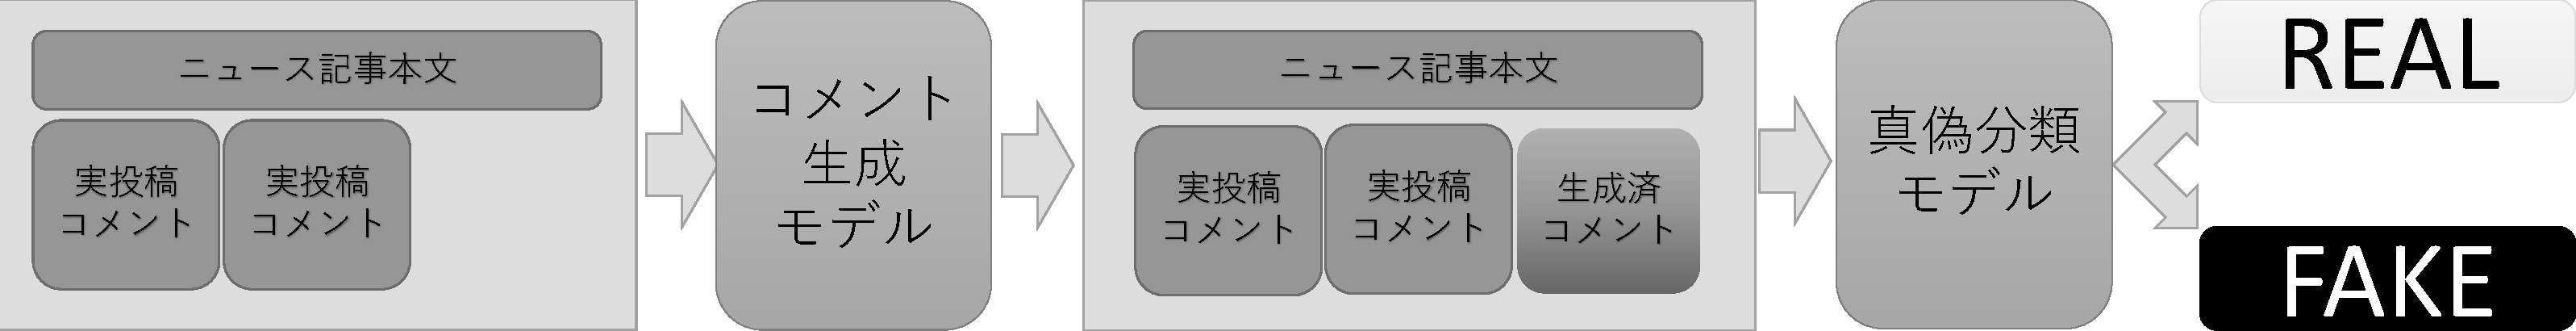
\includegraphics[width=0.95\linewidth]{model.pdf}
		\caption{分類タスクの流れ。コメント生成モデルで1件コメントを生成し真偽分類に活用する。}
		\label{fig:model}
	\end{figure}

	\subsection{特色と独創的な点}
	●\textbf{特色と独創的な点}
	
	\begin{itemize}
		\item 生成タスクを分類タスクに役立てる点
		\item 精度を失わずに速報性をもつことができる点
		\item 生成されたコメントは説明可能性にも役立てられる点
	\end{itemize}

	\subsection{これまでの研究経過及び得られた結果}
	●\textbf{これまでの研究経過及び得られた結果}

	申請者はデータセットとしてFakeNewsNet\cite{Shu2018FakeNewsNetAD}を使用した。
	これはファクトチェックによって\textbf{真偽が評価済である英文ニュース}と、それに\textbf{Twitter上で言及された投稿(ツイート)}等をもつ。
	当研究では最低3件以上英文でコメントとしてツイートが寄せられたニュースを真偽で各2000件使用した。
	拡散の初期段階ではコメントの数は期待できないため、使用するコメントは各3件ずつ無作為に選出し、残りは対象から除外した。

	生成・分類モデルはフェイクニュースを自動で作成するGroverモデル\cite{NIPS2019_9106}を拡張する形で実装した。
	このモデルはフェイクニュースをドメイン・著者・投稿日・見出し・本文の5要素に分け、\textbf{ランダムで歯抜けにして予測させる形で生成学習を実現}したものである。
	今回はこれをユニットの4要素(記事本文と3件のコメント)での実装を目指し調整を行った。
	訓練が完了したコメント生成モデルを使い、図\ref{fig:model}のように\textbf{コメントを1件歯抜けにさせたユニットに生成コメントを付加した上でRealかFakeか分類させた}。
	分類モデルはGroverが提供したものを流用した。

	その結果、生成コメントを含めた場合の\textbf{再現率(Fake記事を見抜いた割合)が0.79}と、歯抜けのまま分類させたときの\textbf{0.75}とコメントなしで分類したときの\textbf{0.62}を上回る結果を得た。
	つまり、コメントを生成することで\textbf{ファクトチェックが必要な疑わしい記事をより多く検出}することができた。

	同時に、生成されたコメントで頻出した単語の傾向において真偽で大きな違いはみられなかった。
	これは、投稿された\textbf{コメントのカテゴリによる出現単語傾向の差は軽微}であることを意味した。

	{\small 
	%\bibliography{myreferences}
	%\bibliographystyle{junsrt}
	\begin{thebibliography}{99}
		\bibitem{agencies_2016} Guardian staff and agencies. Washington gunman motivated by fake news `pizzagate' conspiracy,12 2016.
		\bibitem{ZAROCOSTAS2020676} John Zarocostas. How to fight an infodemic. \textit{The Lancet}, Vol. 395, No. 10225, p. 676, 2020.
		\bibitem{Shu2018FakeNewsNetAD} Kai Shu, Deepak Mahudeswaran, Suhang Wang, Dongwon Lee, and Huan Liu. Fakenewsnet: Adata repository with news content, social context and dynamic information for studying fake newson social media. \textit{ArXiv}, Vol. abs/1809.01286, , 2018.
		\bibitem{NIPS2019_9106} Rowan Zellers, Ari Holtzman, Hannah Rashkin, Yonatan Bisk, Ali Farhadi, Franziska Roesner,and Yejin Choi. Defending against neural fake news. In H. Wallach, H. Larochelle, A. Beygelz-imer, F. d'Alch ́e-Buc, E. Fox, and R. Garnett, editors, \textit{Advances in Neural Information Processing Systems 32}, pp. 9054–9065. Curran Associates, Inc., 2019.
	\end{thebibliography}
	}
	%ぞうの卵はおいしいぞう。
ぞうの卵はおいしいぞう。
ぞうの卵はおいしいぞう。
ぞうの卵はおいしいぞう。
ぞうの卵はおいしいぞう。
ぞうの卵はおいしいぞう。
ぞうの卵はおいしいぞう。
ぞうの卵はおいしいぞう。
ぞうの卵はおいしいぞう。
ぞうの卵はおいしいぞう。
ぞうの卵はおいしいぞう。
ぞうの卵はおいしいぞう。
ぞうの卵はおいしいぞう。
ぞうの卵はおいしいぞう。
ぞうの卵はおいしいぞう。
ぞうの卵はおいしいぞう。
ぞうの卵はおいしいぞう。
ぞうの卵はおいしいぞう。
ぞうの卵はおいしいぞう。
ぞうの卵はおいしいぞう。
ぞうの卵はおいしいぞう。
ぞうの卵はおいしいぞう。
ぞうの卵はおいしいぞう。
ぞうの卵はおいしいぞう。
ぞうの卵はおいしいぞう。
ぞうの卵はおいしいぞう。
ぞうの卵はおいしいぞう。
ぞうの卵はおいしいぞう。
ぞうの卵はおいしいぞう。
ぞうの卵はおいしいぞう。
ぞうの卵はおいしいぞう。
ぞうの卵はおいしいぞう。
ぞうの卵はおいしいぞう。
ぞうの卵はおいしいぞう。
ぞうの卵はおいしいぞう。
ぞうの卵はおいしいぞう。
ぞうの卵はおいしいぞう。
ぞうの卵はおいしいぞう。
ぞうの卵はおいしいぞう。
ぞうの卵はおいしいぞう。
ぞうの卵はおいしいぞう。
ぞうの卵はおいしいぞう。
ぞうの卵はおいしいぞう。
ぞうの卵はおいしいぞう。
ぞうの卵はおいしいぞう。
ぞうの卵はおいしいぞう。
ぞうの卵はおいしいぞう。
ぞうの卵はおいしいぞう。
ぞうの卵はおいしいぞう。
ぞうの卵はおいしいぞう。
ぞうの卵はおいしいぞう。
ぞうの卵はおいしいぞう。
ぞうの卵はおいしいぞう。
ぞうの卵はおいしいぞう。
ぞうの卵はおいしいぞう。
ぞうの卵はおいしいぞう。
ぞうの卵はおいしいぞう。
ぞうの卵はおいしいぞう。
ぞうの卵はおいしいぞう。
ぞうの卵はおいしいぞう。
ぞうの卵はおいしいぞう。
ぞうの卵はおいしいぞう。
ぞうの卵はおいしいぞう。
ぞうの卵はおいしいぞう。
ぞうの卵はおいしいぞう。
ぞうの卵はおいしいぞう。
ぞうの卵はおいしいぞう。
ぞうの卵はおいしいぞう。
ぞうの卵はおいしいぞう。
ぞうの卵はおいしいぞう。
ぞうの卵はおいしいぞう。
ぞうの卵はおいしいぞう。
ぞうの卵はおいしいぞう。
ぞうの卵はおいしいぞう。
ぞうの卵はおいしいぞう。
ぞうの卵はおいしいぞう。
ぞうの卵はおいしいぞう。
ぞうの卵はおいしいぞう。
ぞうの卵はおいしいぞう。
ぞうの卵はおいしいぞう。
ぞうの卵はおいしいぞう。
ぞうの卵はおいしいぞう。
ぞうの卵はおいしいぞう。
ぞうの卵はおいしいぞう。
ぞうの卵はおいしいぞう。
ぞうの卵はおいしいぞう。
ぞうの卵はおいしいぞう。
ぞうの卵はおいしいぞう。
ぞうの卵はおいしいぞう。
ぞうの卵はおいしいぞう。
ぞうの卵はおいしいぞう。
ぞうの卵はおいしいぞう。
ぞうの卵はおいしいぞう。
ぞうの卵はおいしいぞう。
ぞうの卵はおいしいぞう。
ぞうの卵はおいしいぞう。
ぞうの卵はおいしいぞう。
ぞうの卵はおいしいぞう。
ぞうの卵はおいしいぞう。
ぞうの卵はおいしいぞう。
ぞうの卵はおいしいぞう。
ぞうの卵はおいしいぞう。
ぞうの卵はおいしいぞう。
ぞうの卵はおいしいぞう。
ぞうの卵はおいしいぞう。
ぞうの卵はおいしいぞう。
ぞうの卵はおいしいぞう。
ぞうの卵はおいしいぞう。
ぞうの卵はおいしいぞう。
ぞうの卵はおいしいぞう。
ぞうの卵はおいしいぞう。
ぞうの卵はおいしいぞう。
ぞうの卵はおいしいぞう。
ぞうの卵はおいしいぞう。
ぞうの卵はおいしいぞう。
ぞうの卵はおいしいぞう。
ぞうの卵はおいしいぞう。
ぞうの卵はおいしいぞう。
ぞうの卵はおいしいぞう。
ぞうの卵はおいしいぞう。
ぞうの卵はおいしいぞう。
ぞうの卵はおいしいぞう。
ぞうの卵はおいしいぞう。
ぞうの卵はおいしいぞう。
ぞうの卵はおいしいぞう。
ぞうの卵はおいしいぞう。
ぞうの卵はおいしいぞう。
ぞうの卵はおいしいぞう。
ぞうの卵はおいしいぞう。
ぞうの卵はおいしいぞう。
ぞうの卵はおいしいぞう。
ぞうの卵はおいしいぞう。
ぞうの卵はおいしいぞう。
ぞうの卵はおいしいぞう。
ぞうの卵はおいしいぞう。
ぞうの卵はおいしいぞう。
ぞうの卵はおいしいぞう。
ぞうの卵はおいしいぞう。
ぞうの卵はおいしいぞう。
ぞうの卵はおいしいぞう。
ぞうの卵はおいしいぞう。
ぞうの卵はおいしいぞう。
ぞうの卵はおいしいぞう。
ぞうの卵はおいしいぞう。
ぞうの卵はおいしいぞう。
ぞうの卵はおいしいぞう。
ぞうの卵はおいしいぞう。
ぞうの卵はおいしいぞう。
ぞうの卵はおいしいぞう。
ぞうの卵はおいしいぞう。
ぞうの卵はおいしいぞう。
ぞうの卵はおいしいぞう。
ぞうの卵はおいしいぞう。
ぞうの卵はおいしいぞう。
ぞうの卵はおいしいぞう。
ぞうの卵はおいしいぞう。
ぞうの卵はおいしいぞう。
  % << only for demonstration. Please delete it or comment it out.	
%end  現在までの研究状況 ====================
}

